%%%%%%%%%%%%%%%%%%%%%%%%%%%%%%%%%%%%%%%%%
% Programming/Coding Assignment
% LaTeX Template
%
% This template has been downloaded from:
% http://www.latextemplates.com
%
% Original author:
% Ted Pavlic (http://www.tedpavlic.com)
%
% Note:
% The \lipsum[#] commands throughout this template generate dummy text
% to fill the template out. These commands should all be removed when 
% writing assignment content.
%
% This template uses a Perl script as an example snippet of code, most other
% languages are also usable. Configure them in the "CODE INCLUSION 
% CONFIGURATION" section.
%
%%%%%%%%%%%%%%%%%%%%%%%%%%%%%%%%%%%%%%%%%

%%%%%%%%%%%%%%%%%%%%%%%%%%%%%%%%%%%%%%%%%%%%%%
% Modified by George Z. Zachos
% on March 28, 2017 for the Parallel Systems
% and Programming course @cse.uoi.gr
%%%%%%%%%%%%%%%%%%%%%%%%%%%%%%%%%%%%%%%%%%%%%%

%----------------------------------------------------------------------------------------
%	PACKAGES AND OTHER DOCUMENT CONFIGURATIONS
%----------------------------------------------------------------------------------------

\documentclass{article}

\usepackage{fancyhdr} % Required for custom headers
\usepackage{lastpage} % Required to determine the last page for the footer
\usepackage{extramarks} % Required for headers and footers
\usepackage[usenames,dvipsnames]{xcolor} % Required for custom colors
\usepackage{graphicx} % Required to insert images
\usepackage{listings} % Required for insertion of code
\usepackage{courier} % Required for the courier font

% Margins
\topmargin=-0.45in
\evensidemargin=0in
\oddsidemargin=0in
\textwidth=6.5in
\textheight=9.0in
\headsep=0.25in

\linespread{1.1} % Line spacing

% Set up the header and footer
\pagestyle{fancy}
\lhead{\hmwkAuthorName} % Top left header
\chead{\hmwkClass: \hmwkTitle} % Top center head
\rhead{\firstxmark} % Top right header
\lfoot{\lastxmark} % Bottom left footer
\cfoot{} % Bottom center footer
\rfoot{Page\ \thepage\ of\ \protect\pageref{LastPage}} % Bottom right footer
\renewcommand\headrulewidth{0.4pt} % Size of the header rule
\renewcommand\footrulewidth{0.4pt} % Size of the footer rule

%\setlength\parindent{0pt} % Removes all indentation from paragraphs

%----------------------------------------------------------------------------------------
%	CODE INCLUSION CONFIGURATION
%----------------------------------------------------------------------------------------

\definecolor{MyDarkGreen}{rgb}{0.0,0.4,0.0} % This is the color used for comments
\lstloadlanguages{C}
\lstset{language=C,
%         commentstyle=\color{magenta}\itshape,
        morekeywords={pthread_t, pthread_cond_t, pthread_mutex_t},
%         keywordstyle=\color{blue},
%         emphstyle=\color{red},
        breaklines,
        basicstyle=\ttfamily,
        stringstyle=\color{magenta},
%         identifierstyle=\color{cyan}
        frame=single, % Single frame around code
        basicstyle=\ttfamily, % Use small true type font
        showstringspaces=false, % Don't put marks in string spaces
        tabsize=5, % 5 spaces per tab
%         morecomment=[l][\color{Blue}]{...}, % Line continuation (...) like blue comment
        numbers=left, % Line numbers on left
        firstnumber=0, % Line numbers start with line 0
        numberstyle=\small\color{Blue}, % Line numbers are blue and small
        stepnumber=1 % Line numbers go in steps of 1
}

% Creates a new command to include a perl script, the first parameter is the filename of the script (without .pl), the second parameter is the caption
\newcommand{\cscript}[2]{
\begin{itemize}
\item[]\lstinputlisting[caption=#2,label=#1]{#1.c}
\end{itemize}
}

\def\code#1{\texttt{#1}}
%----------------------------------------------------------------------------------------
%	DOCUMENT STRUCTURE COMMANDS
%	Skip this unless you know what you're doing
%----------------------------------------------------------------------------------------

% Header and footer for when a page split occurs within a problem environment
\newcommand{\enterProblemHeader}[1]{
\nobreak\extramarks{#1}{#1 continued on next page\ldots}\nobreak
\nobreak\extramarks{#1 (continued)}{#1 continued on next page\ldots}\nobreak
}

% Header and footer for when a page split occurs between problem environments
\newcommand{\exitProblemHeader}[1]{
\nobreak\extramarks{#1 (continued)}{#1 continued on next page\ldots}\nobreak
\nobreak\extramarks{#1}{}\nobreak
}

\setcounter{secnumdepth}{0} % Removes default section numbers
\newcounter{homeworkProblemCounter} % Creates a counter to keep track of the number of problems

\newcommand{\homeworkProblemName}{}
\newenvironment{homeworkProblem}[1][Problem \arabic{homeworkProblemCounter}]{ % Makes a new environment called homeworkProblem which takes 1 argument (custom name) but the default is "Problem #"
\stepcounter{homeworkProblemCounter} % Increase counter for number of problems
\renewcommand{\homeworkProblemName}{#1} % Assign \homeworkProblemName the name of the problem
\section{\homeworkProblemName} % Make a section in the document with the custom problem count
\enterProblemHeader{\homeworkProblemName} % Header and footer within the environment
}{
\exitProblemHeader{\homeworkProblemName} % Header and footer after the environment
}

\newcommand{\problemAnswer}[1]{ % Defines the problem answer command with the content as the only argument
\noindent\framebox[\columnwidth][c]{\begin{minipage}{0.98\columnwidth}#1\end{minipage}} % Makes the box around the problem answer and puts the content inside
}

\newcommand{\homeworkSectionName}{}
\newenvironment{homeworkSection}[1]{ % New environment for sections within homework problems, takes 1 argument - the name of the section
\renewcommand{\homeworkSectionName}{#1} % Assign \homeworkSectionName to the name of the section from the environment argument
\subsection{\homeworkSectionName} % Make a subsection with the custom name of the subsection
\enterProblemHeader{\homeworkProblemName\ [\homeworkSectionName]} % Header and footer within the environment
}{
\enterProblemHeader{\homeworkProblemName} % Header and footer after the environment
}

%----------------------------------------------------------------------------------------
%	NAME AND CLASS SECTION
%----------------------------------------------------------------------------------------

\newcommand{\hmwkTitle}{Homework \#2} % Assignment title
\newcommand{\hmwkDueDate}{Monday,\ May\ 1,\ 2017} % Due date
\newcommand{\hmwkClass}{MYE023} % Course/class
\newcommand{\hmwkClassTime}{} % Class/lecture time
\newcommand{\hmwkClassInstructor}{Vassilios V. Dimakopoulos} % Teacher/lecturer
\newcommand{\hmwkAuthorName}{George Z. Zachos} % Your name

%----------------------------------------------------------------------------------------
%	TITLE PAGE
%----------------------------------------------------------------------------------------

\title{
\vspace{2in}
\textmd{\textbf{\hmwkClass:\ \hmwkTitle}}\\
\normalsize\vspace{0.1in}\small{Due\ on\ \hmwkDueDate}\\
\vspace{0.1in}\large{\textit{\hmwkClassInstructor}}
\vspace{3in}
}

\author{\textbf{\hmwkAuthorName}}
\date{May 1, 2017} % Insert date here if you want it to appear below your name

%----------------------------------------------------------------------------------------

\setcounter{secnumdepth}{3}

\begin{document}

\maketitle

%----------------------------------------------------------------------------------------
%	TABLE OF CONTENTS
%----------------------------------------------------------------------------------------

\newpage
\tableofcontents
\newpage


%+----------------------------------------------------------+
%|                                                          |
%|          EXERCISE #1                                     |
%|                                                          |
%+----------------------------------------------------------+

\section{Exercise \#1}

\subsection{About}
This exercise is about the multiplication of integer $N$x$N$ arrays using the \texttt{OpenMP}
specification. The serial calculation consists of three (3) nested for-loops and the purpose of
this exercise is to parallelize all three, one at a time. The three resulting programs will be
executed using both \code{static} and \code{dynamic} scheduling policies.

\subsection{Experiment details}
The calculation consists of $N^3$ loop iterations ($N$=1024), while the number of threads
used in \code{parallel} regions is four (4) and chunk size is automatically set to default
values.

\subsubsection{System Specifications}
The experiments were conducted on a Dell OptiPlex 7020:
\begin{itemize}
 \item CPU: Intel\textregistered \ Core\texttrademark \ i5-4590 CPU @ 3.30GHz (64 bit)
 \item RAM: 2 DIMMs x4GiB @ 1600MHz DDR3
 \item Cache line size: 64B (in all levels)
 \item Cache associativity:
 \begin{itemize}
  \item L1, L2: 8-way set associative
  \item L3: 12-way set associative
 \end{itemize}
\end{itemize}

\begin{figure}[htbp]
  \centering
  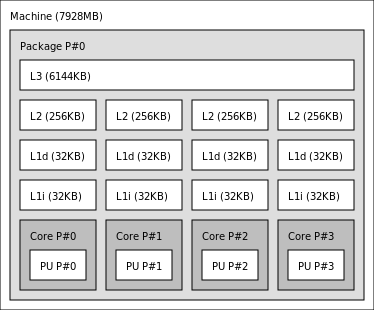
\includegraphics[width=0.5\columnwidth]{./opti7020-topo.png}
  \caption{Topology information of a Dell OptiPlex 7020}
\end{figure}

\pagebreak

\subsection{Timing Results}
In the following table and plot the recorded execution times are displayed.
Note that $X$ axis is plotted on a \underline{linear} scale while $Y$ axis on
a (base 10) \underline{logarithmic} scale.

%------------------------------------ 1

\begin{table}[htbp]
  \centering
    \begin{tabular}{|c||l|l|l|l|l|l|l|l|} 
    \hline
    \multicolumn{4}{|c|}{Timing results of matrix multiplication (Time unit: seconds)} \\
    \multicolumn{4}{|c|}{Array size: 1024x1024, Number of threads: 4} \\
    \hline
    & \multicolumn{3}{|c|}{Parallelized loop nesting level} \\
    \hline
    Scheduling Policy  & \multicolumn{1}{|c|}{0} & \multicolumn{1}{|c|}{1} & \multicolumn{1}{|c|}{2} \\
    \hline\hline
    Static & 0.9228565 & 1.0030725 & 1.988372 \\
    \hline
    Dynamic & 0.87141825 & 1.049885 & 28.30894775 \\
    \hline
    \end{tabular}
  \caption{Timing results of 2D matrix multiplication}
\end{table}


\begin{figure}[htbp]
  \centering
  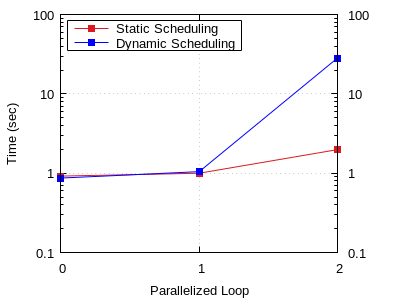
\includegraphics[width=0.55\columnwidth]{../ex1/plots/matmul.png}
  \caption{Timing results of 2D matrix multiplication}
\end{figure}


\subsection{Conclusion}
Based on the results presented above and given that the average execution time of the serial
program is 3,82147025 seconds, we conclude that:

\begin{itemize}
 \item The best program performance\footnote{About 86\% speedup.} is achieved by
       parallelizing the outermost for-loop as only one parallel region is invoked.
       Parallelizing the middle and the innermost loop will cause $N$ and $N^2$
       invocations respectively and the granularity of the tasks being dispatched to
       the team threads to decrease. Due to these continuous invocations, execution
       time is increased as overheads are introduced by thread management (creation, 
       synchronization\footnote{There is an implied barrier at the end of every
       \code{parallel} region.}, destruction etc.).
 \item Both \code{dynamic} and \code{static} schedules result in approximately the
       same execution time, except for the case of parallelizing the innermost 
       for-loop. During \code{static} schedule, the iteration space is divided
       into chunks that are approximately equal in size, and at most one chunk
       is distributed to each thread. In constrast, during \code{dynamic} schedule,
       default chunk size equals to one iteration and in total $N^3$ dispatches
       take place\footnote{$N$ dispatches every time the \code{parallel} construct
       is encountered.}. For this reason, \code{dynamic} schedule exponentially
       increases program time.
\end{itemize}


% %+----------------------------------------------------------+
% %|                                                          |
% %|          EXERCISE #2                                     |
% %|                                                          |
% %+----------------------------------------------------------+
% 
% \section{Exercise \#2}
% 
% \subsection{About}
% This exercise is about the multiplication of integer $N$x$N$ arrays using \texttt{POSIX} threads
% and static scheduling. During static scheduling the parallelizable loops are evenly (when
% possible) divided into chunks of iterations (tasks) and are dispatched to the threads available
% to the runtime system for execution. Due to this even distribution of iterations and in contrast
% to dynamic scheduling, a thread executing on a processor under heavy workload will have a lower
% throughput capability and will lead to an increase of the total execution time. The purpose of
% this exercise is to parallelize only the \underline{outermost} for-loop of the serial calculation,
% time the matrix multiplication and observe how altering the number of threads will affect execution
% time.
% 
% \subsection{Implementation details}
% If $T$ is the number of threads, and $N$ is the array dimension, then the outermost
% for-loop of the serial program consists of $N$ iterations, that should be divided
% into $T$ chunks. When $T$ divides $N$ evenly, the exact chunk size is $N/T$. In the
% opposite case, $S=N \bmod T$ threads will be assigned $\lfloor{N/T}\rfloor+1$ iterations
% and $T-S$ threads will be assigned $\lfloor{N/T}\rfloor$ iterations. We are going
% to refer to $S$ as the number of special threads because these threads execute one
% more iteration than the rest. This policy manages to avoid a lopsided distribution
% of iterations to threads as it may increase workload by only a single iteration
% \footnote{This additional iteration may add significant delays in coarse-grained
% tasks}.
% 
% \newpage
% 
% \subsection{Experiment details}
% During this experiment, thread number takes value in \{1, 2, 4, 8, 12, 16\} and array
% size is 1024x1024.
% 
% \subsubsection{System Specifications}
% The experiments were conducted again on a Dell OptiPlex 7020.
% 
% 
% \subsection{Timing Results}
% In the following table and plot the recorded execution times are displayed.
% Note that $X$ axis is plotted on a (base 2) \underline{logarithmic} scale while
% $Y$ axis on a \underline{linear} scale.
% 
% %------------------------------------ 1
% 
% \begin{table}[htbp]
%   \centering
%     \begin{tabular}{|c||l|l|l|l||l|} 
%     \hline
%     \multicolumn{6}{|c|}{Timing results of matrix multiplication (Time unit: seconds)} \\
%     \multicolumn{6}{|c|}{Array size: 1024x1024} \\
%     \hline
%    \# of threads & 1st run & 2nd run & 3rd run & 4th run & Average time\\ [0.5ex] 
%     \hline\hline
%     1 & 5.057095 & 4.319662 & 3.157559 & 5.297035 & 4.45783775 \\ 
%     \hline
%     2 & 2.648351 & 2.545161 & 1.940197 & 2.043663 & 2.294343 \\
%     \hline
%     4 & 0.918773 & 0.800195 & 1.504583 & 1.504583 & 1.07884625 \\
%     \hline
%     8 & 0.971947 & 1.428921 & 1.224236 & 0.990774 & 1.1539695 \\
%     \hline
%     12 & 0.965793 & 0.986273 & 0.981548 & 1.130868 & 1.0161205 \\
%     \hline
%     16 & 1.208460 & 1.241845 & 1.015431 & 0.974093 & 1.10995725 \\ [1ex]
%     \hline
%     \end{tabular}
%   \caption{Timing results of 2D matrix multiplication}
% \end{table}
% 
% 
% \begin{figure}[htbp]
%   \centering
%   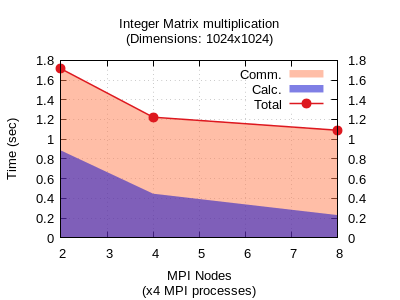
\includegraphics[width=0.55\columnwidth]{../ex2/plots/matmul.png}
%   \caption{Timing results of 2D matrix multiplication}
% \end{figure}
% 
% %------------------------------------
% \pagebreak
% 
% \subsection{Conclusion}
% Based on the results presented above and given that the average execution time of the serial
% program is 4,297561 seconds, we conclude that:
% 
% \begin{itemize}
%  \item Program performance is approximately doubled as the number of threads is increased, until
%        oversubscription bottleneck is hit and execution time becomes almost constant
%        \footnote{This is also the conclusion we came to on Exercise \#1}.
%  \item Execution time of the parallel program when a single thread is used to perform the
%        calculation is a bit higher than the time of the serial program. Moreover, we observed
%        that execution time in general varies from time to time. Several reasons such as context
%        switching, thread affinity, cache misses \& cache pollution justify the existence of
%        these overheads and consequently this behavior.
% \end{itemize}


%+----------------------------------------------------------+
%|                                                          |
%|          EXERCISE #3                                     |
%|                                                          |
%+----------------------------------------------------------+

\section{Exercise \#3}

\subsection{About}
This exercise is about the multiplication of integer $N$x$N$ arrays using \texttt{OpenMP} tasks
and checkerboard partitioning. During checkerboard partitioning, the initial matrix is divided
into submatrices of size $S$x$S$. The purpose of this exercise is to assign the calculation
of each submatrix to an \texttt{OpenMP} task and observe how altering the number of tasks
will affect execution time.

\subsection{Experiment details}
During this experiment, the number of \texttt{OpenMP} tasks takes value in \{16, 256, 1024\},
initial array size is 1024x1024 and the number of threads used in \code{parallel} regions is
four (4).

\subsubsection{System Specifications}
The experiments were conducted again on a Dell OptiPlex 7020.

\subsection{Timing Results}
In the following table and plot the recorded execution times are displayed.
Note that $X$ axis is plotted on a (base 2) \underline{logarithmic} scale while
$Y$ axis on a \underline{linear} scale.

\begin{table}[htbp]
  \centering
    \begin{tabular}{|c||l|l|l|l||l|} 
    \hline
    \multicolumn{6}{|c|}{Timing results of matrix multiplication (Time unit: seconds)} \\
    \multicolumn{6}{|c|}{Array size: 1024x1024} \\
    \hline
   \# of \texttt{OpenMP} Tasks & 1st run & 2nd run & 3rd run & 4th run & Average time\\ [0.5ex] 
    \hline\hline
    16 & 0.798303 & 0.790874 & 1.156564 & 0.901301 & 0.9117605 \\ 
    \hline
    256 & 1.003373 & 0.993386 & 0.863506 & 0.974971 & 0.958809 \\
    \hline
    1024 & 1.191109 & 1.036035 & 1.138259 & 0.956815 & 1.0805545 \\ [1ex]
    \hline
    \end{tabular}
  \caption{Timing results of 2D matrix multiplication using \texttt{OpenMP}
           tasks and checkerboard partitioning}
\end{table}


\begin{figure}[htbp]
  \centering
  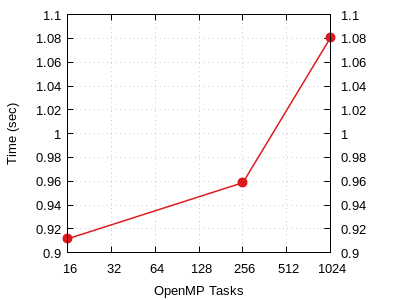
\includegraphics[width=0.55\columnwidth]{../ex3/plots/matmul.png}
  \caption{Timing results of 2D matrix multiplication using \texttt{OpenMP}
           tasks and checkerboard partitioning}
\end{figure}


\subsection{Conclusion}
Based on the results presented above and given that the average execution time of the serial
program is 3,82147025 seconds, we conclude that:

\begin{itemize}
 \item Program performance is decreased as the number of \texttt{OpenMP} tasks is increased.
       This happens due to the overheads related to task management (creation,
       task switching etc.).
 \item Even though overheads related to task management are introduced, execution time remains
       significantly lower compared to the one of the serial program. This is because
       the significant synchronization overheads\footnote{As observed in Exercise \#1 where
       the increase of \code{parallel} region encounters results in a linear increase of
       the number of implicit barriers.} do not increase relatively to the task number.
       Actually no syncrhonization takes place at all except for the implicit barrier
       at the end of the \code{parallel} region.
\end{itemize}

\end{document}